\documentclass[tikz,border=2pt]{standalone}
\usepackage{amsmath}
\usetikzlibrary{arrows.meta}
\begin{document}
% K_x = floor(T_x): every death time in [k, k+1) gives K_x = k; a death at T_x = 3.7 gives K_x = 3
% and an end-of-year death payment at time K_x + 1 = 4.
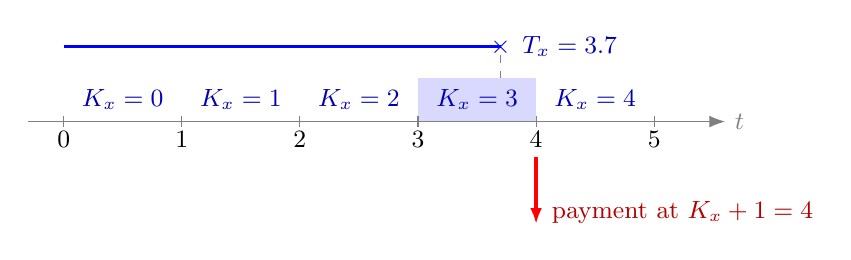
\begin{tikzpicture}[font=\small, >={Latex[length=2mm]}, x=1.5cm, y=1cm]
  \fill[blue!15] (3,0) rectangle (4,0.55);
  \draw[gray, ->] (-0.3,0) -- (5.6,0) node[right] {$t$};
  \foreach \k in {0,...,5} {
    \draw[gray] (\k,-0.07) -- (\k,0.07);
    \node[below, inner sep=2pt] at (\k,-0.05) {$\k$};
  }
  \foreach \k in {0,...,4} \node[blue!70!black] at (\k+0.5,0.28) {$K_x=\k$};
  % the life, ending at T_x = 3.7
  \draw[blue, very thick] (0,0.95) -- (3.7,0.95);
  \node[blue] at (3.7,0.95) {$\times$};
  \node[blue!70!black, anchor=west] at (3.8,0.95) {$T_x=3.7$};
  \draw[gray, thin, dashed] (3.7,0.85) -- (3.7,0.55);
  % end-of-year payment
  \draw[->, red, very thick] (4,-0.45) -- (4,-1.3);
  \node[red!70!black, anchor=west] at (4.05,-1.15) {payment at $K_x+1=4$};
\end{tikzpicture}
\end{document}
